% CHAPTER 2: Overview of transformer architecture
\chapter{A high-level overview of the Transformer architecture}

Given below is an architecture of a transformer as mentioned in the original paper:
\begin{figure}[h]
    \centering
    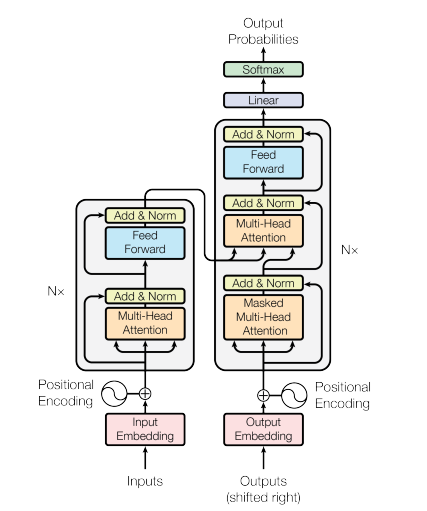
\includegraphics[width=0.4\linewidth]{High-level-overview/transformer-architecture.png}
    \caption{Transformer architecture}
\end{figure}

Most of you will be thinking to stop reading this report after looking at this figure! But don't worry! We will simplify each and every component of this diagram and understand how all of them work together. By the end, you will have a clear picture of a transformer in mind and will be confident enough to teach this concept to someone else.\\

A transformer can be thought of as a black box that takes an input, does some processing and gives an output. In the example provided below, it translates a sentence from one language to another.\\

\begin{figure}[H]
    \centering
    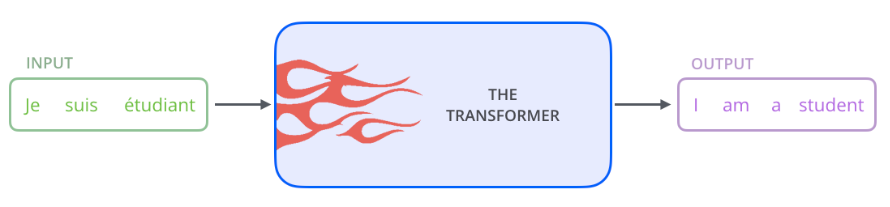
\includegraphics[width=0.5\linewidth]{High-level-overview/simplified.png}
\end{figure}

If we peek into the black box, then a simplified representation of the components can be drawn.
\begin{figure}[H]
    \centering
    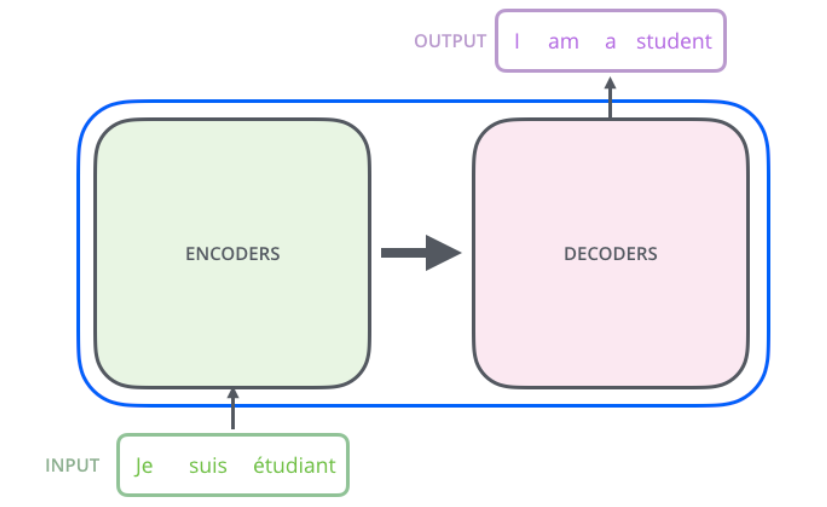
\includegraphics[width=0.4\linewidth]{High-level-overview/encoder-decoder.png}
    \caption{A simplified representation of the Transformer architecture}
\end{figure}

What is interesting is that there is not one encoding and decoding block, but many of them stacked one above the other. That is what the \textbf{N$\times$} means in the original architecture. In the original paper, the researchers used 6 of them.
\begin{figure}[H]
    \centering
    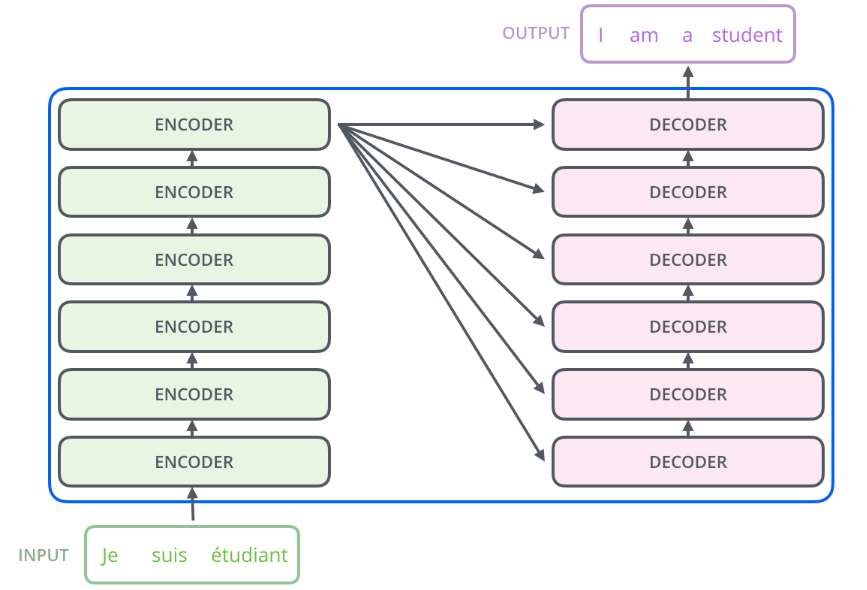
\includegraphics[width=0.35\linewidth]{High-level-overview/encoder-decoder-multiple.png}
    \caption{Multiple encoding and decoding blocks stacked one above the other}
\end{figure}

All the encoder and decoder blocks are identical in terms of their architecture but contain different values of parameters. We will discuss later what these parameters are. If we zoom in a little on the blocks, then they appear as follows: \\
\begin{figure}[H]
    \centering
    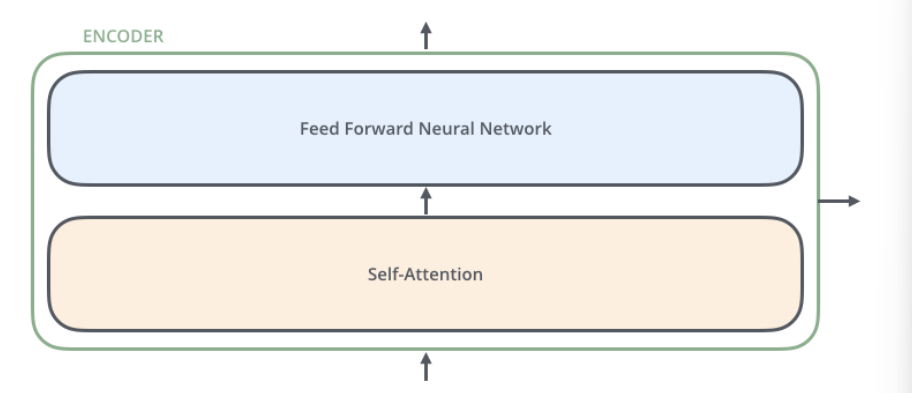
\includegraphics[width=0.35\linewidth]{High-level-overview/encoder-simplified.png}
    \caption{A simplified version of the encoder and decoder blocks}
\end{figure}

Don't worry about what all the components are at this point. We are only having a rough idea of what is there inside. From the next chapter onward, we will delve into the various components of this architecture.
